\documentclass[11pt,letterpaper]{article}

% Paquetes básicos
\usepackage[utf8]{inputenc}
\usepackage[T1]{fontenc}
\usepackage[margin=2.5cm]{geometry}
\usepackage{graphicx}
\usepackage{xcolor}
\usepackage{array}
\usepackage{booktabs}
\usepackage{colortbl}
\usepackage{fancyhdr}
\usepackage{titlesec}
\usepackage{enumitem}
\usepackage{siunitx}
\usepackage{hyperref}
\usepackage{float}
\usepackage{amssymb}
\usepackage{tikz} 
\usepackage{caption} % Agregado para poder usar caption sin numeración

% Configuración de colores
\definecolor{navy}{HTML}{003366}
\definecolor{royal}{HTML}{0055A4}
\definecolor{success}{HTML}{2E8B57}
\definecolor{lightgray}{HTML}{F0F2F5}

% Configuración de hipervínculos
\hypersetup{colorlinks=true, linkcolor=navy, urlcolor=royal}

% Ajuste encabezado
\setlength{\headheight}{23pt}

% Encabezados globales
\pagestyle{fancy}
\fancyhf{}
\fancyhead[L]{\small\textcolor{navy}{\textbf{INGENIERÍA DE VALOR: CASO DE ÉXITO}}}
\fancyhead[R]{\small\textcolor{gray}{Eficiencia Térmica Industrial}}
\fancyfoot[C]{\thepage}
\renewcommand{\headrulewidth}{0.5pt}
\renewcommand{\headrule}{\hbox to\headwidth{\color{royal}\leaders\hrule height \headrulewidth\hfill}}

% Títulos
\titleformat{\section}{\Large\bfseries\color{navy}}{}{0em}{}[\titlerule]
\titleformat{\subsection}{\large\bfseries\color{royal}}{}{0em}{}

% Espaciado
\setlength{\parskip}{0.8em}
\setlength{\parindent}{0pt}

\begin{document}

% ============================================================
% PÁGINA 1: PORTADA
% ============================================================
\thispagestyle{empty}

\begin{center}
    \vspace*{1cm}
    {\Large\textcolor{gray}{INFORME DE INGENIERÍA DE DETALLE}}\\[0.5cm]
    {\Huge\textbf{\textcolor{navy}{SISTEMA DE RECUPERACIÓN DE CALOR (HRS)}}}\\[0.5cm]
    {\Large\textcolor{royal}{\textbf{Optimización Energética en Compresores de Aire}}}\\[2cm]
\end{center}

% Caja de Impacto
\begin{center}
\fcolorbox{navy}{lightgray}{%
    \begin{minipage}{0.9\textwidth}
        \vspace{0.5cm}
        \centering
        \Large\textbf{\textcolor{navy}{IMPACTO DEL PROYECTO}}\\[0.5cm]
        
        \begin{tabular}{rl}
            \textbf{Potencia Recuperada:} & \textbf{622 kW} (Térmicos) \\
            \textbf{Eficiencia del Sistema:} & 96\% \\
            \textbf{Periodo de Retorno:} & \huge\textcolor{success}{\textbf{< 2 meses}} \\
            \textbf{Disponibilidad:} & 8.000 horas/año \\
            \textbf{Reducción CO$_2$:} & 1.232 ton/año \\
        \end{tabular}
        \vspace{0.5cm}
    \end{minipage}
}
\end{center}

\vspace{1.5cm}

\section*{EL EQUIPO: SIMULACIÓN + EJECUCIÓN}
La clave del éxito no fue solo la tecnología, sino una ingeniería de detalle que eliminó los sobrecostos típicos de instalación y aseguró la fiabilidad operativa desde el día 1.

\vspace{0.5cm}

\begin{tabular}{p{0.45\textwidth} | p{0.45\textwidth}}
    \textbf{\textcolor{navy}{Nilton Martínez}} & \textbf{\textcolor{navy}{Felipe Wasaff}} \\
    \textit{Ing. Climatización y Automatización} & \textit{Físico Computacional} \\
    \footnotesize
    \textbf{Rol:} Ingeniería de Detalle, Hidráulica y Control. Diseño de estrategias modulares para mantenimiento cero-paradas. & 
    \footnotesize
    \textbf{Rol:} Simulación Térmica y Modelamiento. Validación de escenarios de carga parcial y optimización de intercambio. \\
    \href{https://www.linkedin.com/in/nilton-martinez-a0168131/}{[Ver LinkedIn]} & \href{https://www.linkedin.com/in/felipewasaff/}{[Ver LinkedIn]} \\
\end{tabular}

\vfill
\begin{center}
    \small\textcolor{gray}{Documento de Portafolio Técnico -- Datos Anonimizados\\
    Fecha del Proyecto: Diciembre 2024}
\end{center}

\newpage

% ============================================================
% PÁGINA 2: DESAFÍO Y SOLUCIÓN
% ============================================================

\section{DESAFÍO Y SOLUCIÓN TÉCNICA}

\subsection{El Problema}
Una planta industrial desperdiciaba energía térmica en sus 6 compresores de aire (1.200 kW instalados). El desafío era capturar este calor para procesos sin afectar la contrapresión ni la operación crítica de los compresores.

\subsection{La Solución: Ingeniería a Medida}
Desarrollamos un sistema ``Plug \& Play'' a nivel de procesos, priorizando la estabilidad hidráulica y la facilidad de mantenimiento.

\begin{table}[h]
\centering
\small
\renewcommand{\arraystretch}{1.2}
\begin{tabular}{@{}ll@{}}
\toprule
\textbf{Variable} & \textbf{Especificación Técnica} \\
\midrule
Capacidad de Diseño & 622 kW térmicos recuperados \\
Delta T Proceso & Elevación de 35$^{\circ}$C a 70$^{\circ}$C \\
Tecnología HX & Placas Alfa Laval CB30 (+38\% factor ensuciamiento) \\
Bombeo & \textbf{Modular: 6 x Grundfos TPE3} (Redundancia N+1 implícita) \\
Control & Lazo PID autónomo con integración a SCADA planta \\
\bottomrule
\end{tabular}
\end{table}

\subsection{Ingeniería de Valor Agregado}

\textbf{1. Simulación Computacional (Python):}
Modelamos 7 escenarios de operación (desde 16\% hasta 100\% de carga). Esto nos permitió dimensionar los equipos con precisión quirúrgica, evitando el sobredimensionamiento que usualmente encarece estos proyectos en un 20-30\%.

\textbf{2. Fiabilidad Hidráulica y Modularidad:}
En lugar de grandes bombas centralizadas, optamos por una arquitectura distribuida (1 bomba micro por compresor).
\begin{itemize}[leftmargin=*, label=$\checkmark$]
    \item \textbf{Eficiencia Energética:} Solo operan las bombas de los compresores activos. Eliminación total de consumo parásito en carga parcial.
    \item \textbf{Mantenimiento sin Paradas:} Se utiliza equipamiento estandarizado (\textit{commodity}). Ante una falla, el reemplazo se realiza en minutos con repuestos de bajo costo, sin detener la planta, eliminando la dependencia de equipos costosos hechos a medida.
    \item \textbf{Seguridad:} Balance de presiones validado para evitar cavitación a altas temperaturas.
\end{itemize}

% Salto de página para el diagrama a pantalla completa
\newpage

% ============================================================
% PÁGINA 3: DIAGRAMA P&ID (A PANTALLA COMPLETA)
% ============================================================

% Cambiamos la geometría SOLO para esta página (Márgenes CERO absolutos)
\newgeometry{left=0cm, right=0cm, top=0cm, bottom=0cm}
\thispagestyle{empty} % Quitamos encabezado y pie de página para ganar espacio

\begin{figure}[p]
    \centering
    % angle=90 rota la imagen
    % width=0.95\paperheight hace que el ancho (que ahora es alto) ocupe casi toda la hoja
    % keepaspectratio asegura que no se deforme
    % IMPORTANTE: Asegúrate de tener 'pid_diagram.png' en la carpeta
    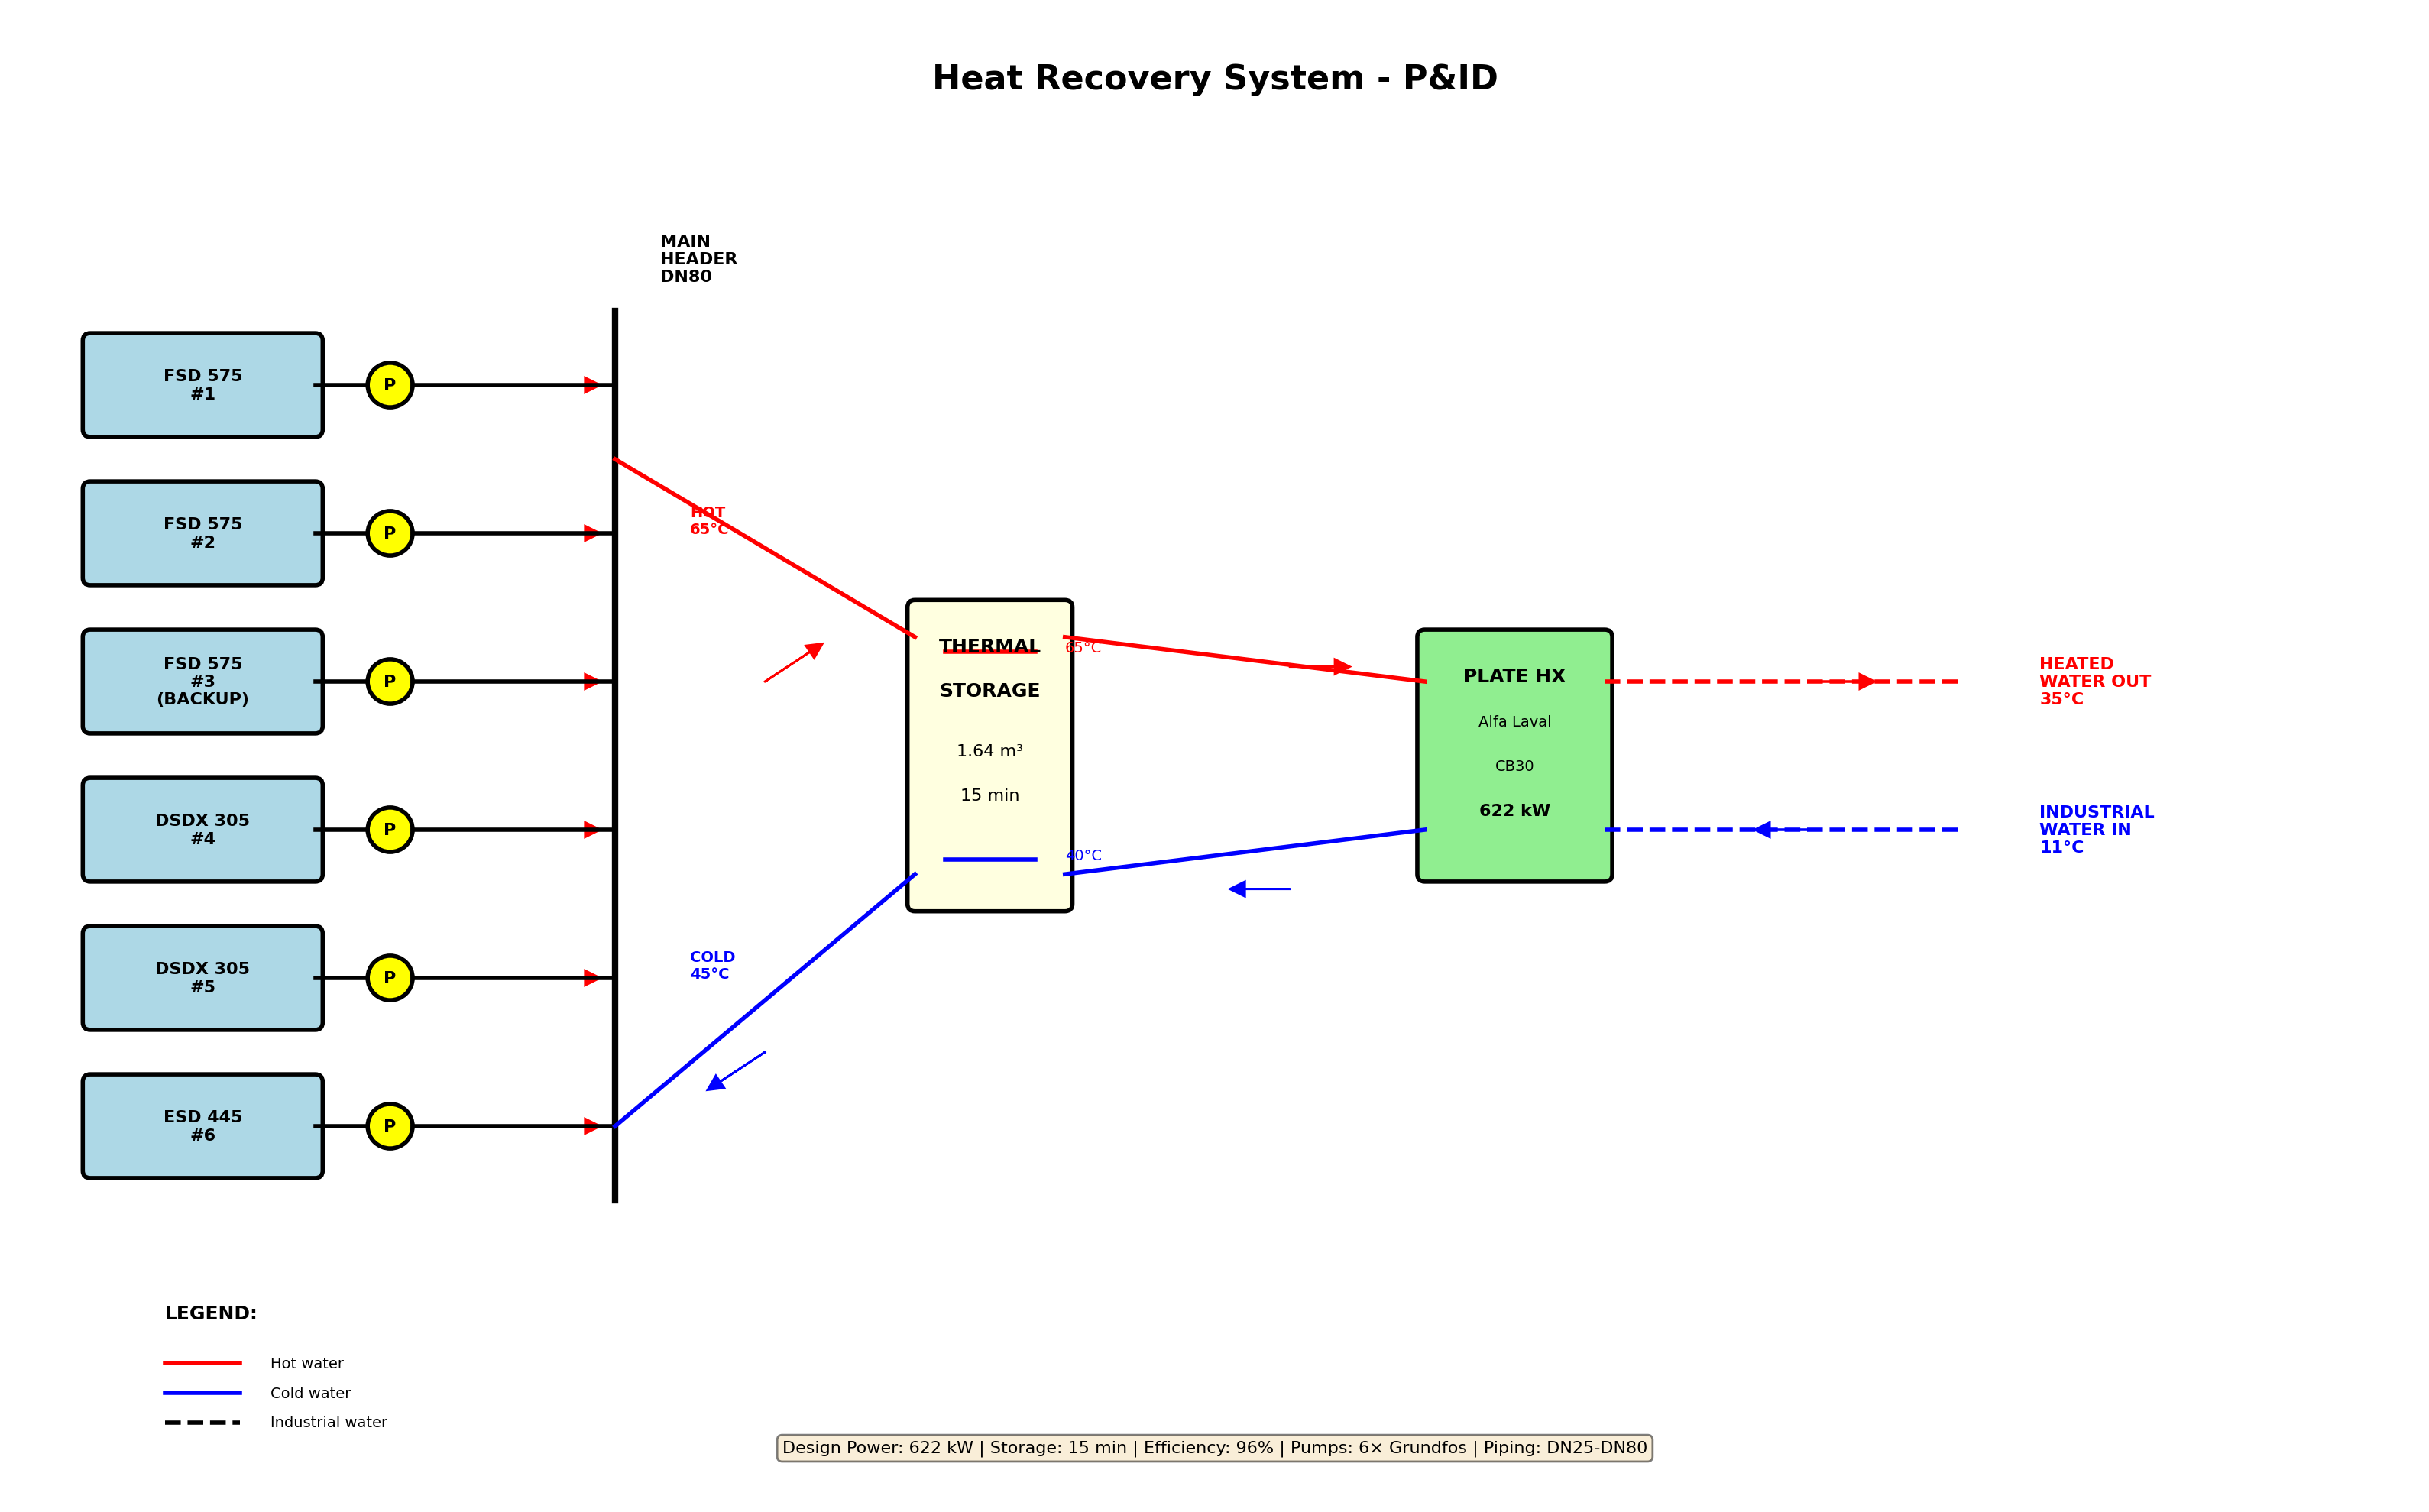
\includegraphics[angle=90, width=0.6\paperheight, keepaspectratio]{pid_diagram.png}
\end{figure}

% Restauramos la geometría normal para las siguientes páginas
\restoregeometry

\newpage

% ============================================================
% PÁGINA 4: RESULTADOS
% ============================================================

\section{RESULTADOS OPERACIONALES}

Más allá de la recuperación de calor, el éxito del proyecto radica en su integración transparente con la operación existente y su impacto ambiental inmediato.

\subsection{Indicadores de Desempeño (KPIs)}

El sistema demostró un desempeño superior a las expectativas teóricas gracias al ajuste fino realizado durante la ingeniería de detalle.

\begin{itemize}[itemsep=10pt]
    \item \textbf{Velocidad de Retorno (Payback):}
    Debido a la alta utilización (24/7) y al diseño optimizado en costos (sin sobredimensionamiento), la inversión se recuperó en \textbf{menos de 60 días} de operación plena.
    
    \item \textbf{Eficiencia Térmica:}
    El sistema opera con una eficiencia de transferencia del \textbf{96\%}, maximizando el aprovechamiento de la energía que antes se disipaba a la atmósfera.
    
    \item \textbf{Impacto Ambiental:}
    La reducción de consumo de combustible fósil en calderas se traduce directamente en una huella de carbono menor.
\end{itemize}

\vspace{1.5cm}

\subsection{Sostenibilidad Verificable}

\begin{center}
    \begin{tikzpicture}
        % Círculo CO2
        \node[circle, draw=success, line width=1mm, minimum size=3.5cm, align=center, fill=success!10] at (0,0) {\textbf{1.232}\\\small Ton CO$_2$/año\\\small Evitadas};
        
        % Círculo Equivalencia
        \node[circle, draw=navy, line width=1mm, minimum size=3.5cm, align=center, fill=navy!10] at (6,0) {\textbf{4.976}\\\small MWh/año\\\small Recuperados};
        
        % Texto conector
        \draw[->, thick, gray, line width=2pt] (2,0) -- (4,0);
        \node[above, gray] at (3,0) {\small Equivale a};
    \end{tikzpicture}
\end{center}

\vspace{1cm}

\section{CONCLUSIONES}

\subsection{¿Por qué funcionó este proyecto?}
\begin{enumerate}
    \item \textbf{Ingeniería ``EPC Ready'':} Entregamos planos y especificaciones listos para construir, eliminando ambigüedades que generan sobrecostos en obra.
    \item \textbf{Decisiones Basadas en Datos:} No usamos estimaciones empíricas. Simulamos la termodinámica real del proceso para cada punto de operación.
    \item \textbf{Enfoque en Mantenibilidad:} Diseñamos pensando en el operador que tendrá que mantener el sistema en 5 años más.
\end{enumerate}

\vspace{1.5cm}

\begin{center}
    \rule{0.6\textwidth}{0.5pt}
    
    \vspace{0.5cm}
    
    {\Large \textbf{¿Energía residual en su proceso?}}
    
    \vspace{0.3cm}
    
    Transformamos pérdidas técnicas en ganancias operativas.\\
    Realizamos diagnósticos preliminares para identificar su potencial.
    
    \vspace{1cm}
    
    \textbf{\Large CONVERSEMOS}
    
    \vspace{0.3cm}
    
    \begin{tabular}{c c}
        \textbf{Nilton Martínez} & \textbf{Felipe Wasaff} \\
        \small Ingeniero de Proyectos & \small Especialista en Simulación \\
    \end{tabular}
    
    \vspace{0.5cm}
    \small\textit{\#IngenieriaDeDetalle \#EficienciaEnergetica \#CalorResidual}
\end{center}

\end{document}